\documentclass[10pt]{article}
\usepackage[margin=2.2cm]{geometry}
\usepackage{graphicx}
\usepackage{booktabs}
\usepackage{amsmath}
\usepackage{amssymb}
\usepackage{xcolor}
\usepackage[hidelinks]{hyperref}
\setlength{\parskip}{4pt}
\setlength{\parindent}{0pt}
\graphicspath{{../../../output/01_romallosa/}}

\newcommand{\ok}{\textcolor{green!55!black}{\checkmark}}
\newcommand{\res}[1]{\textcolor{orange!80!black}{#1}}

\title{\vspace{-1.2cm}\textbf{Review 01 --- Romallosa 2003 replication}\\
\large \texttt{mcdo\_dev} Phase 1 \quad(\texttt{output/01\_romallosa/},
\texttt{docs/theory/01\_richards\_wolf\_pulse.md})}
\author{}
\date{2026-06-12}

\begin{document}
\maketitle
\vspace{-1.1cm}

\section*{Engine and validated conventions}

Richards--Wolf integrals $I_0,I_1,I_2$ (paper Eqs.~5--7); intensity cut
$|I_0-I_2|^2$ ($x$-polarized beam, scan $\perp$ polarization, $\phi=\pi/2$) ---
the only cut with true zeros, required by the paper's ``cw contains zero
points''. Pulsed intensity = Eq.~10 spectral sum, \textbf{201 frequencies over
the full positive spectrum $\omega\in(0,2\omega_c)$}. This window is the
critical convention: the literal FWHM-band reading of the paper's text discards
24\% of the spectral weight and gives $S_{tr}=1.020$ vs the paper's 1.062.
Implemented as half-width $\min(4\sigma,\omega_c)$ in \texttt{config.omega\_grid()}.

Further conventions established numerically:
the paper's Fig.~2 \emph{panel labels are swapped} (its ``r $\pm6\,\mu$m'' panel
is the axial profile, zeros at $\pm3.05\,\mu$m); Fig.~3's energy fraction is a
\emph{1-D line integral} over the 201-point array (cylindrical gives 0.46 ---
wrong); Linfoot arrays sample in \emph{optical coordinates}
($v\in\pm6.70$, $u\in\pm24.74$), which is what makes $F,S$ NA-flat;
Fig.~1 axes are $r\pm2.0$, $z\pm6.0\,\mu$m (scan lost the decimals).

\section*{Scorecard}

\begin{center}
\small
\begin{tabular}{llll}
\toprule
Figure & paper anchor & ours & status\\
\midrule
1 & cw island contours / pulsed smooth barrel & same topology & \ok\\
2 & zeros $0.555/3.05\,\mu$m; pedestal $\approx0.1$ / $0.05$ & $0.555/3.05$; $0.13$ / $0.049$ & \ok\\
3 & plateau $\approx0.78$; $0.65$ @ 1 fs; linear $\tau\le2$ fs & $0.777$; $0.62$ & \ok~\res{$-3\%$ @1 fs}\\
4 & $S_{ax}{=}1.057$, $S_{tr}{=}1.062$, $F{\approx}0.96$, NA-flat & $1.058$, $1.053$, $0.96$, flat & \ok~\res{$S_{tr}-0.9\%$}\\
5 & $S(1\,\mathrm{fs})$ on $0.97\tau^{0.04}$ & $0.970$ & \ok~exact\\
\bottomrule
\end{tabular}
\end{center}

Residuals trace to conventions the paper never documents (exact array windows,
RK4 quadrature). CW anchors: transverse FWHM 472.8 nm, axial 2419 nm.

\textbf{Bugs found in old mcdo} (fixed on its \texttt{cleanup} branch,
commit \texttt{695f9da}): spectral power $\sqrt2$ too narrow (double-squaring
--- 1 fs behaved as 1.4 fs); library window truncated at the FWHM; circular
polarization cannot reproduce the zero structure.

\clearpage
\begin{center}
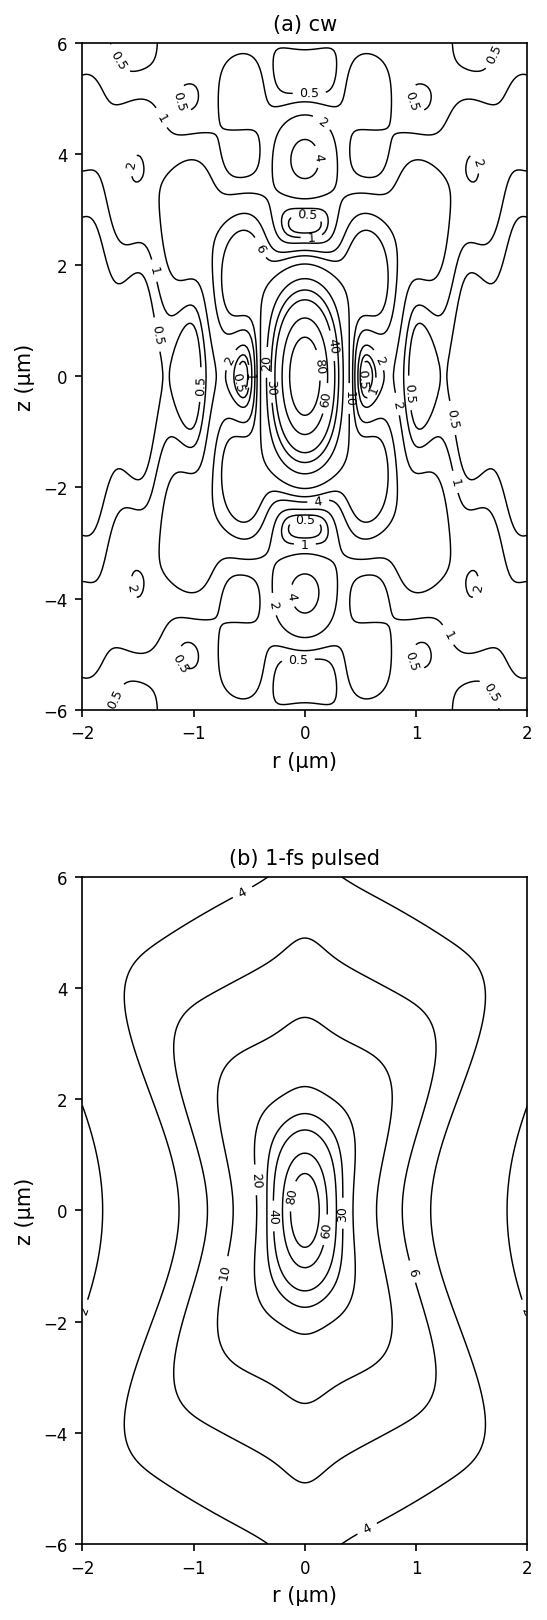
\includegraphics[width=0.42\textwidth]{fig1_contours.png}
\end{center}
\textbf{Fig.~1} --- cw panel: island-contour topology produced by the zero
structure (axial sidelobe islands, diagonal ridges); pulsed panel: smooth
barrel, zeros filled by spectral averaging. Matches the paper's Fig.~1 layout
on $r\pm2.0$, $z\pm6.0\,\mu$m.

\begin{center}
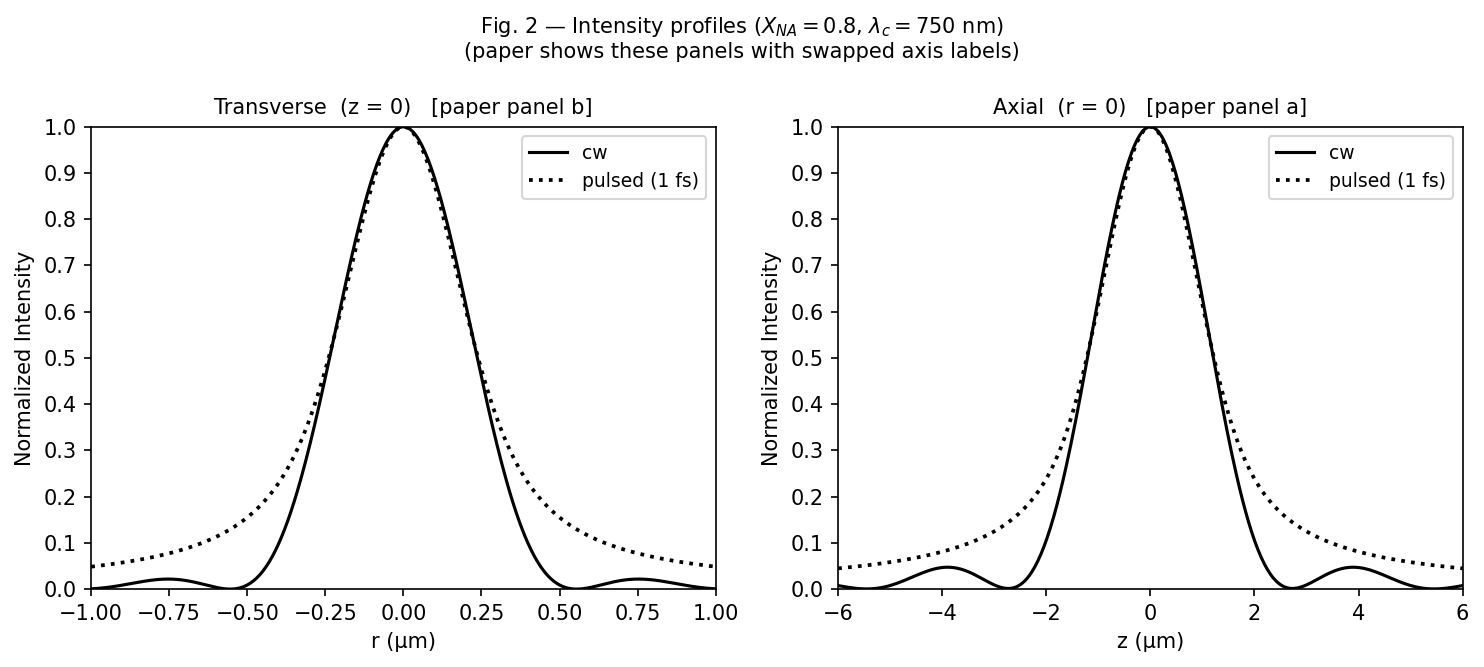
\includegraphics[width=0.95\textwidth]{fig2_profiles.png}
\end{center}
\textbf{Fig.~2} --- cw (solid) with true zeros at $0.555\,\mu$m (transverse)
and $3.05\,\mu$m (axial); pulsed (dotted) pedestal $\approx0.13$ at the zero
ring, $0.049$ at $r=1\,\mu$m (paper $\approx0.1$/$0.05$). FWHM 472.8 nm cw /
479.0 nm pulsed.

\clearpage
\begin{center}
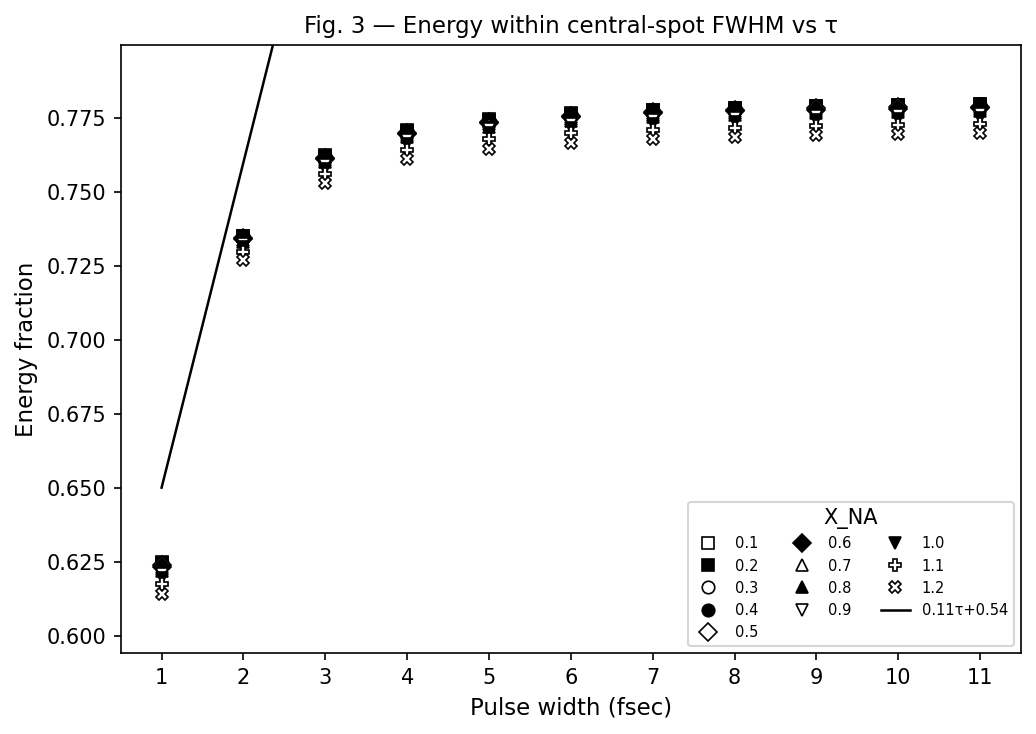
\includegraphics[width=0.60\textwidth]{fig3_energy.png}
\end{center}
\textbf{Fig.~3} --- energy within the central-spot FWHM (1-D definition):
plateau 0.777, sharp linear drop below $\tau=2$ fs to 0.62 at 1 fs, reference
line $0.11\tau+0.54$ valid only $\tau\lesssim2$ fs; tight NA clustering with
$X_{NA}=1.2$ lowest --- all as published.

\begin{center}
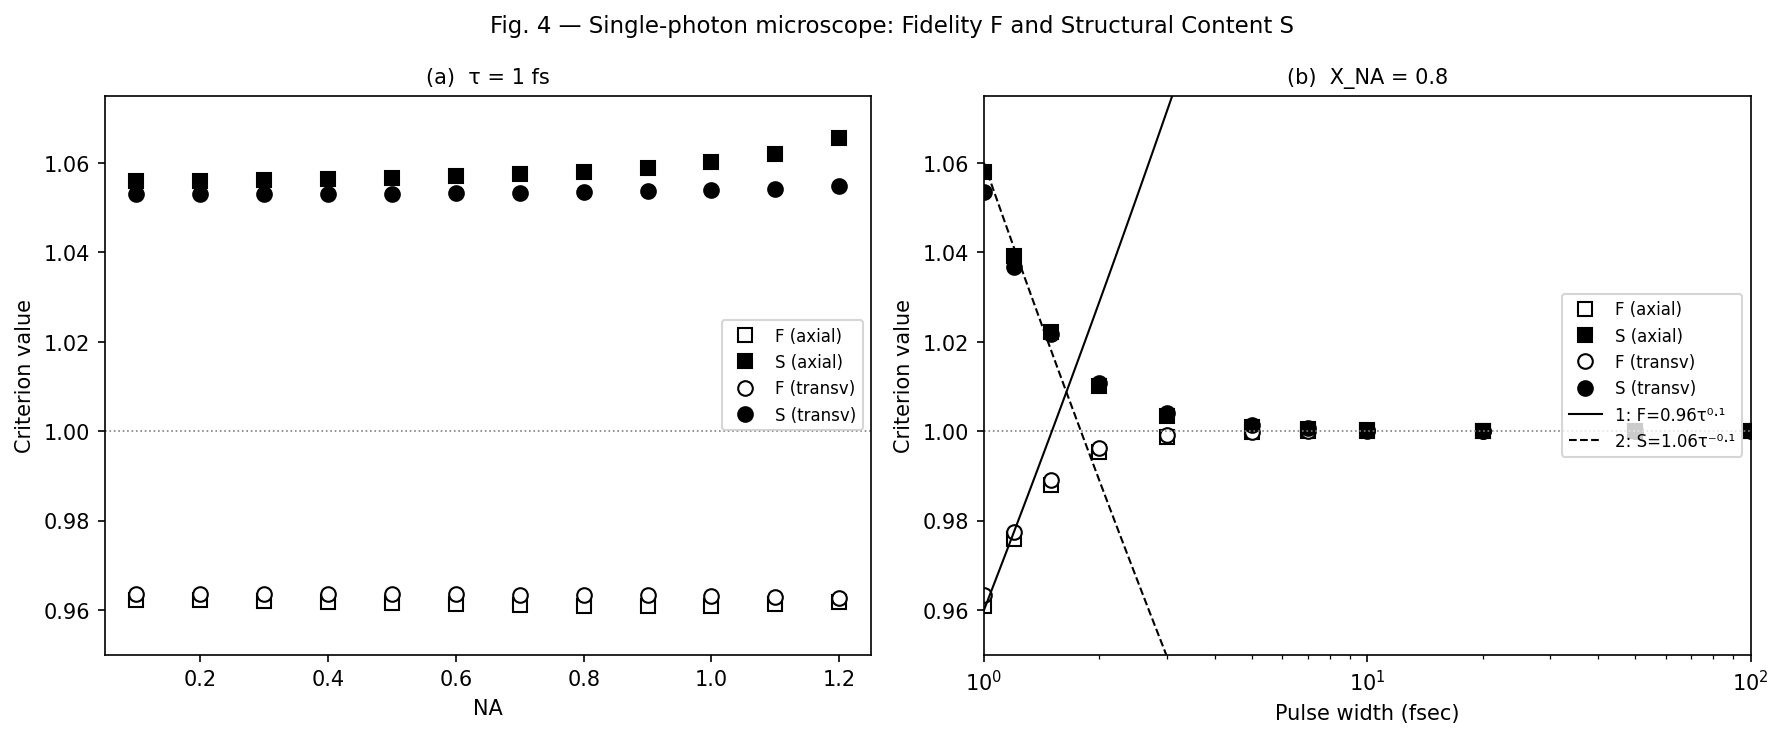
\includegraphics[width=0.95\textwidth]{fig4_linfoot.png}
\end{center}
\textbf{Fig.~4} --- (a) $F$ and $S$ flat across $X_{NA}=0.1$--$1.2$ at
$\tau=1$ fs ($S_{ax}$ mean 1.058 vs paper $1.057\pm0.0018$); (b) sudden
deterioration below $\tau=1.2$ fs, data hugging the caption's
$F=0.96\tau^{0.1}$, $S=1.06\tau^{-0.1}$ near 1--2 fs.

\begin{center}
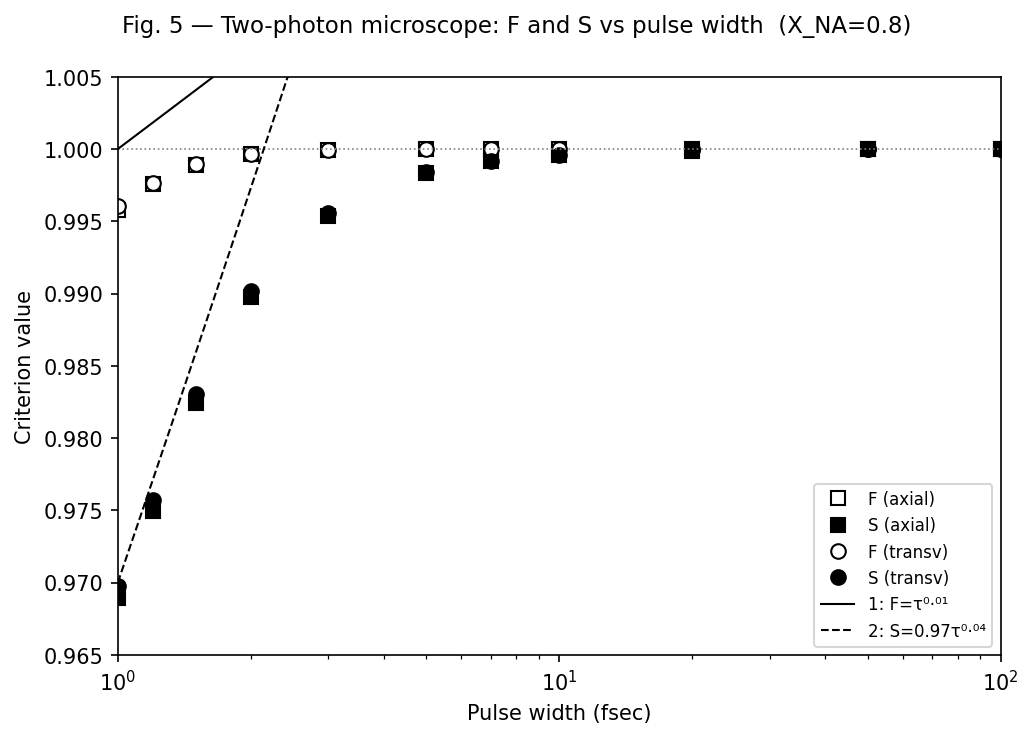
\includegraphics[width=0.60\textwidth]{fig5_linfoot_2p.png}
\end{center}
\textbf{Fig.~5} --- two-photon PSF $=$ (normalized $|E|^2$)$^2$:
$S(1\,\mathrm{fs})=0.970$, exactly on the caption's $0.97\tau^{0.04}$;
two-photon deterioration ($\approx3\%$) weaker than single-photon
($\approx5$--$6\%$) --- the paper's headline conclusion, reproduced.

\end{document}
